\chapter{Desarrollo}
\label{chap:desarrollo}

El desarrollo del software producto de este trabajo, se realizó en el idioma Inglés debido a que todos los documentos en los que se basa el modelo de conocimiento están escritos en ese idioma y la realización de una traducción de dichos documentos escapa al alcance de este trabajo, además, muchos de los términos utilizados día a día en el campo de las Ciencias de la Computación son provenientes del Inglés y muchos no tienen una traducción aceptada y que mantenga coherencia con el término original. Todo esto aunado a que la mayor parte de la información novedosa en el campo de las Ciencias de la Computación se escribe primero en Inglés y, posteriormente, se traduce a otros idiomas, causaría más impacto la liberación de una herramienta en Inglés que en Español, es por ello que, tanto la interface gráfica como la documentación, fueron desarrollados y escritos en Inglés.

El desarrollo de este trabajo, se describe siguiendo la metodología planteada anteriormente. Las iteraciones citadas en el \textit{Marco Metodológico} serán descritas a continuación de manera consecutiva:

\section{[Iteración 1]: Investigación y análisis}
Durante esta etapa no se desarrolló ningún tipo de software, es por ello que no se verán historias de usuario, diseño, desarrollo ni pruebas unitarias.

\subsection{Desarrollo de las tareas}
Las tareas de esta iteración se basaron principalmente en la investigación y profundización de los temas relacionados a este trabajo, así como la búsqueda de herramientas para el ensamblaje de la plataforma de desarrollo.

\subsubsection{Investigación de los temas relacionados}
La mayor parte de la investigación realizada fue descrita en el \textit{Marco Teórico} del presente trabajo. El tópico central del presente trabajo resulta ser \textit{La Web Semántica}, por ello, es necesario tomar en cuenta todos los conceptos que se desprenden de dicho tópico. Los conceptos más importantes que se desprenden de \textit{La Web Semántica} son citados a continuación:

\begin{itemize}
\item Ontologías o modelos de conocimiento.
\item Motores de inferencia.
\end{itemize}

Las \textit{Ontologías} o \textit{Modelos de conocimiento}, son el eje central de la \textit{Web Semántica}. Es lo que establece toda la estructura de meta-datos en la que se basa el etiquetado e indexado de los recursos que forman parte de la base de conocimientos. Además, establece las relaciones entre las meta-entidades que conforman la \textit{Ontología}. Define el vocabulario que modela el dominio del problema a ser resuelto.

Los \textit{Motores de inferencia} son herramientas que, dadas ciertas reglas sobre un \textit{modelo de conocimiento}, son capaces de deducir nueva información y nuevas relaciones entre las meta-entidades y, por lo tanto, nuevas relaciones entre los recursos dentro de la base de conocimientos.

\subsubsection{El problema y los requerimientos}
Del problema general del proyecto, puede plantearse como se presenta a continuación: \textit{¿Cómo facilitar el acceso a la información acerca de Ciencias de la Computación a personas interesadas en el área?}. De este problema, puede identificarse los siguientes requerimientos:

\begin{itemize}
\item Una interfaz web donde los usuarios puedan interactuar con el sistema.
\item Una interfaz de edición que permita a usuarios autorizados agregar nuevos recursos y extender la base de conocimiento.
\item Una interfaz de edición que permita a usuarios autorizados agregar meta-información nueva y extender el modelo de conocimiento.
\item Un componente de traducción que convierta consultas en lenguaje semi-natural a SPARQL, el lenguaje de consultas sobre RDF/RDFS/OWL.
\item Desarrollo de un modelo de conocimiento del área de Ciencias de la Computación e Ingeniería Informática.
\item Un componente capaz de realizar consultas e inferencias sobre el modelo de conocimiento realizado.
\end{itemize}

\subsubsection{Selección de la plataforma}
Al principio, se planteó llevar a cabo todo el desarrollo utilizando \textit{Python} como lenguaje de programación y las librerías nativas disponibles a través de \textit{easy\_install}, pues \textit{Python} es uno de los pocos lenguajes que ofrece librerías nativas para la manipulación de documentos RDF, además de las ventajas propias que ofrece el lenguaje desde el punto de vista sintáctico y de facilidad de aprendizaje y de programación. Pero a la hora de buscar Frameworks que permitieran el desarrollo de aplicaciones basadas en Web Semántica y Motores de Inferencia, la información y la cantidad de herramientas resultó limitada.

Debido a la situación expuesta en el párrafo anterior, se planteó seleccionar la mejor herramienta para cada uno de los componentes del sistema, es decir, la mejor plataforma para la \textit{herramienta para la administración de la ontología} y la mejor plataforma para el buscador como tal.

\subsubsection{Herramienta para la administración de la ontología}
Las dos opciones más fuertes para el desarrollo de este componente fueron \textit{Python} por un lado, por ser una plataforma 100\% libre y de código abierto y por la gran cantidad de librerías disponibles para extender el lenguaje, y por otro lado \textit{Java} representaba una opción viable, por ser una plataforma con más de 15 años de desarrollo y estándar \textit{de-facto} de la industria, a continuación se presentan las características más destacables de cada una de las opciones:

\begin{itemize}
\item \textbf{Python:} según la \textit{Python Software Foundation}, el lenguaje cuenta con las siguientes características
    \begin{itemize}
    \item Totalmente abierto y libre.
    \item Sintaxis clara y legible.
    \item Capacidad poderosa de introspección.
    \item Multiparadigma: funcional, estructurado y orientado a objetos.
    \item Tipos de dato dinámicos.
    \item Gestión de errores basada en excepciones.
    \item Puede extenderse a través de la escritura de módulos en lenguaje C o C++.
    \item Gran cantidad de librerías, entre ellas varias para procesar documentos RDF.
    \item Facilidad para operar con otras plataformas.
    \item Precompilado y semi-interpretado.
    \end{itemize}

\item \textbf{Java:} según Joyanes y Zahonero (2002), \textit{Java}, es un lenguaje que posee las siguientes características
    \begin{itemize}
    \item Sencillo, fue diseñado para facilitar las tareas del programador profesional.
    \item Orientado a objetos.
    \item Distribuido, facilita el desarrollo de aplicaciones que hacen uso de la red mediante la incorporación de clases que manejan protocolos TCP/IP.
    \item Precompilado y semi-interpretado.
    \item Arquitectura neutra, debido a que se ejecuta en una máquina virtual.
    \item Portable, dado que al ``compilar'' no se produce un archivo ejecutable como ocurre en los lenguajes compilados (como C, C++ y Pascal, por ejemplo), sino un \textit{bytecode} que es ejecutado por la máquina virtual, este \textit{bytecode} puede ser ejecutado en cualquier otro sistema operativo, siempre y cuando exista en él una instancia de la \textit{Máquina Virtual de Java}.
    \item Multihilo, un programa en \textit{Java} puede ejecutar múltiples tareas de manera simultánea
    \end{itemize}
\end{itemize}

Ambas plataformas ofrecen prestaciones muy similares, si bien el núcleo de \textit{Python} no es muy amplio, posee gran cantidad de librerías para extender su funcionalidad. De igual manera, \textit{Java} incorpora cientos de clases que lo convierten en un lenguaje amplio y poderoso.

Para este componente, se decidió trabajar con \textit{Java}, ya que, como se verá más adelante, ofrece el mejor Framework para el desarrollo de aplicaciones basadas en Web Semántica y, al seleccionar dicho Framework, la transitividad conduce a trabajar con este lenguaje.

\subsubsection{Buscador}
El buscador, es el encargado de realizar peticiones al motor de consultas sobre RDF e interactuar con el usuario final, es por ello que la generación de vistas es un aspecto importante en esta parte del sistema.

Para el desarrollo de la herramienta de búsqueda, fue seleccionada la plataforma \textit{Python}, debido a todas las razones expuestas anteriormente, además de contar con una gran cantidad de \textit{frameworks} y herramientas que facilitan el desarrollo web.

\subsubsection{Selección de los Frameworks de desarrollo}
Luego de realizar una investigación en la web, los Frameworks de desarrollo que parecen ser más utilizados para las aplicaciones semánticas son:

\begin{itemize}
    \item \textbf{Sesame:} escrito en \textit{Java}.
    \item \textbf{RedLand:} escrito en C y accesible desde \textit{Python} mediante \textit{Wrapping}.
    \item \textbf{Jena:} escrito en \textit{Java}.
    \item \textbf{CubicWeb:} escrito en \textit{Python}.
\end{itemize}

En este caso, se tomó la decisión de trabajar con el Framework \textit{Jena} debido a que es el que ofrece la mayor cantidad de documentación disponible en línea, además, es compatible con todos los niveles de representación semántica de meta-información (RDF, RDFS y OWL), posee varios motores de inferencia ya integrados y permite la integración con motores de inferencia externos, tiene un motor de consultas SPARQL y ofrece la posibilidad de integrarse con medios de persistencia externos, además de ser libre y de código abierto (The Jena Community, s/f), sin embargo, los razonadores incluíos en \textit{Jena} no son compatibles con OWL, por ello se seleccionó \textit{Pellet}, un motor de inferencia externo al Framework, escrito en \textit{Java} y compatible con \textit{Jena}.

El Framework \textit{Sesame}, ofrece prestaciones técnicas similares a las de \textit{Jena}, sin embargo, la documentación disponible en línea no es comparable con la que ofrece este último y, a pesar de ser de código abierto, es propiedad de una empresa alemana llamada \textit{ADUNA} (Autor desconocido, s/f) y para poder acceder a información más profunda o solicitar ayuda en algo relacionado al Framework, es necesario pagar por horas de consultoría, lo que hace poco viable la utilización de \textit{Sesame} para este proyecto.

\textit{RedLand}, escrito en C y accesible desde \textit{Python}, según la comunidad \textit{RedLand} (s/f), luego de leer la documentación, es compatible sólo con RDF y, para este trabajo, el modelo de conocimientos planteado utilizaría anotaciones definidas en la especificación RDFS y, posiblemente, algunas definidas en el dialecto OWL-Lite, por lo que fue descartado. Además, el proceso de instalación y configuración resulta complicado comparado al de las otras opciones.

Finalmente \textit{CubicWeb}, a pesar de ser un Framework realmente completo pues ofrece toda la plataforma para el desarrollo: desde la persistencia, hasta la generación de vistas, pero fue descartado por no ser compatible con SPARQL, sino con su antecesor: RQL (CubicWeb Community, s/f).

\subsubsection{Selección del medio de persistencia}
Para la persistencia de datos, si bien los manejadores de base de datos relacionales tradicionales como MySQL y Postgres ofrecen paquetes para la gestión de documentos RDF y OWL, existe una alternativa que ofrece dicha funcionalidad de manera nativa. Se trata de \textit{Virtuoso}, un manejador de base de datos con capacidad de gestionar información en formato RDF y XML, compatible con los estándares ODBC y JDBC, posee un motor de inferencia interno, puede correr en ambientes federados, según información de la comunidad (Virtuoso Community, s/f) y, además, existe una edición \textit{Open Source} bastante completa y muy bien documentada.

\section{[Iteración 2]: Diseño de la arquitectura del sistema}
El sistema estará constituido por dos aplicaciones distintas. La primera, escrita en \textit{Java}, constituye una herramienta de administración para la ontología, la segunda, desarrollada en \textit{Python} constituye una interfaz de consultas sobre la ontología. El servidor, está constituido por el motor de persistencia que, simplemente, almacenará el modelo una vez aplicado el razonamiento a través de un motor de inferencia. Además, se cuenta con una estructura de archivos expuesta vía HTTP a través de Apache, en la que se encuentra el modelo original y el modelo razonado para ser consumidos por cualquier otra aplicación que desee hacer uso de la ontología, bien sea para aplicar razonamiento al modelo base o para hacer uso del modelo razonado y sus recursos.

A continuación se presenta el diagrama de arquitectura resultante del análisis previo:

\begin{figure}[h!]
    \begin{center}
        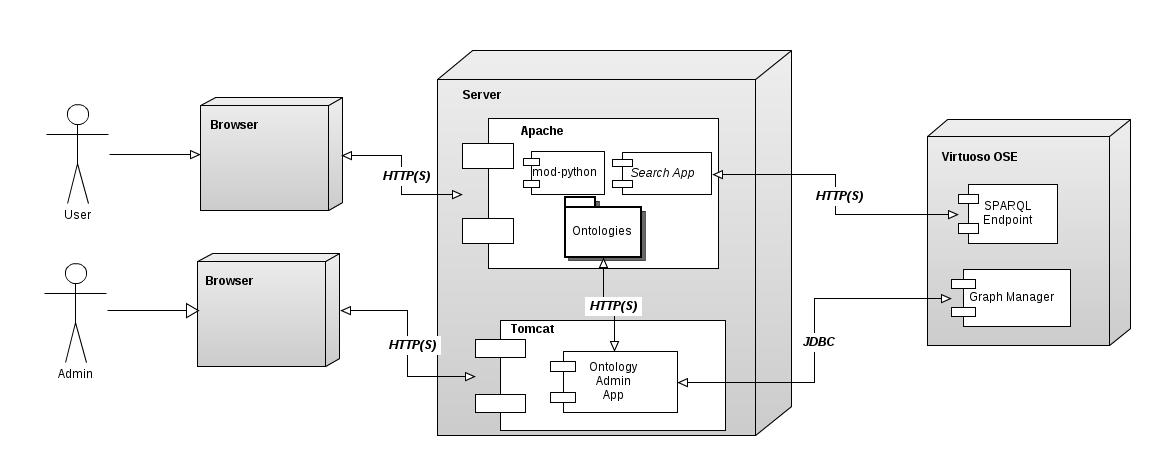
\includegraphics[scale=0.4]{images/sysArch.jpg}
        \caption{Arquitectura del sistema}
        \label{systemArchitecture}
    \end{center}
\end{figure}

\section{[Iteración 3]: Establecimiento del ambiente de desarrollo}
En esta iteración no se desarrolló ningún tipo de software, por ello, no fue necesaria la realización de pruebas unitarias, sin embargo, se llevó a cabo un proceso de configuración posterior a la selección de las herramientas de desarrollo.

\subsection{Desarrollo de las tareas}
El proceso que dirigió la etapa de desarrollo, fué el proceso de programación o codificación, en dos lenguajes de programación distintos: \textit{Python} del lado del \textit{Cliente} y \textit{Java} del lado del \textit{Servidor}, es por ello que el \textit{Sistema Operativo} utilizado en el equipo de desarrollo y despliegue del sistema, \textbf{debe} facilitar la instalación y configuración de las herramientas necesarias para realizar dicho trabajo, además de albergar el sistema una vez desarrollado.

A nivel de \textit{Sistema Operativo}, se seleccionó una distribución de \textit{GNU/Linux}, muy popular en el mundo de los desarrolladores de software y servidores, ya que ofrece compatibilidad con \textit{Java} a través de una instancia de la máquina virtual y el intérprete de \textit{Python} usualmente viene preinstalado en todos los sistemas \textit{GNU/Linux}. La distribución seleccionada fue \textit{Debian} pues, ofrece alrededor de 30.000 paquetes de software instalables a través del gestor de paquetes \textit{aptitude} o, su front-end gráfico \textit{Synaptic} (Debian Community, s/f), además, las versiones de esta distribución de \textit{GNU/Linux} usualmente tienen años de diferencia pues la comunidad pone especial atención en liberar software que está 100\% probado y estable (Autor Desconocido, 2011).

A nivel de servidores de aplicaciones, se seleccionó \textit{Tomcat} para alojar la aplicación \textit{servidora} por ser estándar \textit{de-facto} en la industria a la hora de alojar aplicaciones web desarrolladas en \textit{Java} y \textit{Apache2} para alojar la aplicación \textit{cliente}, junto con \textit{libapache-mod-python} para activar la compatibilidad del servidor \textit{Apache2} con \textit{Python}.

Para desarrollar las tareas de programación, se seleccionaron las siguientes herramientas:
\begin{itemize}
    \item Para desarrollar en \textit{Java}, se seleccionó el Entorno Integrado de Desarrollo (IDE) \textit{Eclipse}
    \item La \textit{Ontología}, ya que debe ser escrita en RDF/OWL, se seleccionó el editor \textit{Protègè}, desarrollado en la Universidad de Stanford, este editor, permite el modelado de manera gráfica y la generación automática de código válido en varias sintaxis de RDF/OWL.
    \item Para desarrollar en \textit{Python}, los requerimientos no son muchos, por ello, para mantenerlo simple, se seleccionó el editor \textit{VIM}, con el \textit{plugin} NERDTree, que permite la visualización de la estructura de directorios del proyecto y la apertura de varios archivos de código fuente en distintas pestañas a nivel de terminal.

\subsubsection{Configuración}
Toda la instalación de los paquetes necesarios para el desarrollo, a excepción de los \textit{plugins} para \textit{VIM} y los entornos de desarrollo \textit{Eclipse} y \textit{Protègè}, fueron descargados, instalados y configurados a través del gestor de paquetes de Debian.

En el caso de \textit{Eclipse}, no hizo falta instalarlo, pues la comunidad provee un paquete que ejecuta la aplicación, con el único requisito de tener \textit{Java} instalado. Lo mismo ocurrió en el caso de \textit{Protègè}.

\section{[Iteración 4] Análisis y desarrollo de la \textit{ontología}}
Durante esta iteración, si bien se desarrolló una parte importante del sistema como lo es la \textit{ontología}, no se codificó software como tal. La etapa de pruebas unitarias, fue sustituida por una etapa de validación del modelo de conocimiento.

\subsection{Desarrollo de las tareas}
Para el desarrollo de la \textit{ontología} definitiva, fue necesario realizar un análisis previo para determinar cómo está estructurado el conocimiento en las áreas de \textit{Ciencias de la Computación} e \textit{Ingeniería Informática}, posteriormente, se procedió a realizar el diseño, codificación y validación de la \textit{ontología} hasta llegar al modelo final.

\subsubsection{Análisis}
Antes de realizar un diseño preliminar de la \textit{ontología}, es necesario realizar un análisis de la estructura del conocimiento en el área, con este análisis se busca:

\begin{enumerate}
    \item Establecer las \textit{entidades} que conformarán la \textit{ontología}.
    \item Determinar las \textit{relaciones} existentes entre las \textit{entidades}.
    \item Determinar las \textit{propiedades} de las \textit{relaciones} existentes entre las \textit{entidades}.
    \item Conocer más a fondo el dominio del problema a ser resuelto.
\end{enumerate}

El item número uno, se refiere a determinar las clases \textit{RDF} que conformarán el modelo de conocimiento. A través del número dos, se desea obtener la \textit{jerarquía de clases} de las entidades junto con las relaciones entre ellas a través de \textit{RDFS}, es decir, si se hace analogía con el esquema Orientado a Objetos, se busca obtener el \textit{modelo de dominio} del problema. El punto número tres, hace referencia a las propiedades y condiciones de las relaciones definidas en el punto anterior, es decir, a través del vocabulario \textit{OWL Lite}, definir las reglas de inferencia sobre las relaciones del modelo a través de las propiedades lógicas de transitividad, simetría y reflexividad, así como también la definición de propiedades inversas. El cuarto y último punto, se refiere a conocer a fondo cómo está compuesto el conocimiento en el área que es objeto de estudio, en este caso, \textit{Ciencias de la Computación}.

Los cuatro (4) ítem enumerados anteriormente, pueden resumirse como \textit{Determinar la estructura del conocimiento en el área seleccionada}. Para ello, es necesario aplicar técnicas de \textit{Ingeniería del Conocimiento}. Según Norvig y Rusell (2004) \textit{Ingeniero de Conocimiento}, es alguien que investiga un dominio concreto, aprende qué conceptos son los importantes de ese dominio y crea una representación formal de los objetos y relaciones del dominio. En este caso, el dominio ya ha sido investigado por el autor durante los años de carrera, simplemente hace falta determinar qué conceptos son importantes en el área y producir la representación formal de dichos conceptos y las relaciones que guardan entre sí.

\subsubsection{Diseño}
Luego de analizar el área seleccionada y con base en las recomendaciones de la \textit{IEEE Computer Society} (IEEE-CS) y la \textit{Assosiation for Computing Machinery} (ACM), descritas en los documentos \textit{Computing Curricula 2001, Computer Science Final Report} (IEEE-CS y ACM, 2001) y el \textit{Computer Science Curriculum 2008: An Interim Revision of CS 2001} (ACM, 2008) para el campo de las \textit{Ciencias de la Computación} y el documento \textit{Computer Engineering 2004: Curriculum Guidelines for Undergraduate Programs in Computer Engineering} (IEEE-CS, 2004), que incorpora elementos de Ingeniería al primero, se llegó a la estructura jerárquica de clases mostrada en la Figura~\ref{classHierarchy}:


\begin{figure}[h!]
    \begin{center}
        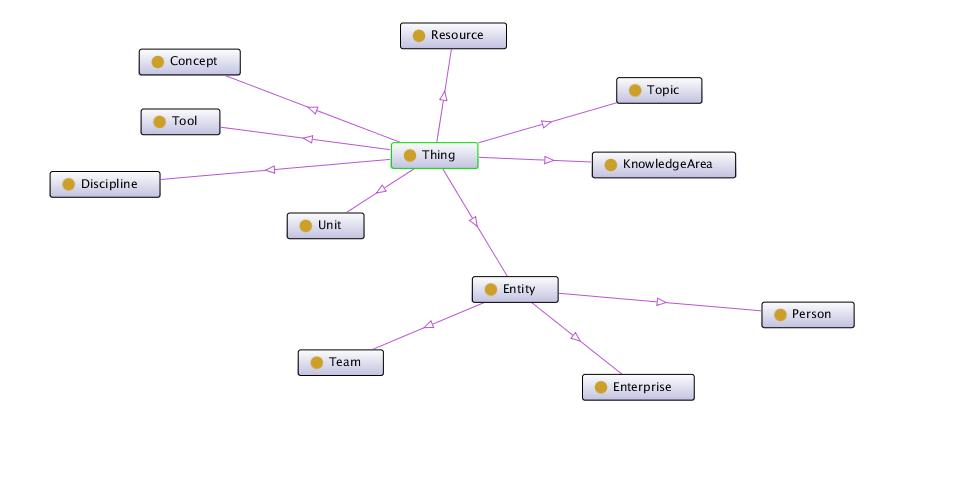
\includegraphics[scale=0.5]{images/onto_graph_classes.jpg}
        \caption{Jerarquía de clases}
        \label{classHierarchy}
    \end{center}
\end{figure}

En RDF/OWL, todas las clases o entidades heredan por defecto de la clase \textit{Thing}, un principio similar al de la clase \textit{Object} en \textit{Java}, las líneas moradas expresan precisamente eso, una relación de \textit{herencia} entre dos entidades que puede leerse como \textit{is-a} (\textit{es-un} o \textit{es-una}), esta relación de \textit{herencia} es, además, transitiva, lo que nos permite inferir, por ejemplo, que un elemento de la clase \textit{Person}, es también un \textit{Thing} aunque no exista una relación directa, pues la clase de nivel inmediatamente superior lo es. Las clases \textit{KnowledgeArea}, \textit{Unit} y \textit{Topic}, son las mismas utilizadas en los documentos de la \textit{IEEE-CS} y la \textit{ACM} para dividir los grandes bloques de conocimiento, en unidades más pequeñas, manejables y específicas a cada nivel como se muestra en la Figura~\ref{knowledgeStructure}. La clase \textit{Discipline}, fue agregada para hacer referencia al marco global del problema cuyo dominio se está modelando, en este caso \textit{Ciencias de la Computación}, con el objetivo de facilitar la adaptación de este modelo a otros dominios. Por otra parte, la clase \textit{Concept}, fue agregada con el propósito de lograr una granularidad más fina y poder expresar niveles de conocimiento más específico, las clases \textit{Entity}, \textit{Person}, \textit{Team}, \textit{Resource} y \textit{Enterprise} serán explicadas posteriormente.

\begin{figure}[h!]
    \begin{center}
        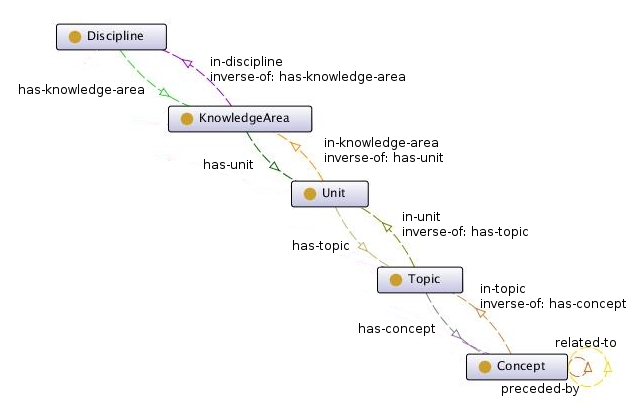
\includegraphics[scale=0.5]{images/onto_knowledge_structure.jpg}
        \caption{Estructura del conocimiento según \textit{IEEE-CS} y \textit{ACM}}
        \label{knowledgeStructure}
    \end{center}
\end{figure}

En la Figura~\ref{knowledgeStructure} se muestra la estructura del conocimiento según las recomendaciones de la \textit{ACM} y la \textit{IEEE-CS}, puede observarse que es una estructura de \textit{Contención} o \textit{Agregación}, donde el nivel superior contiene todo lo que se encuentra en los niveles inferiores y, análogamente, los niveles inferiores conforman su nivel inmediatamente superior. También, según la Figura~\ref{knowledgeStructure}, las propiedades a la derecha (las que tienen el prefijo \textit{in}) son propiedades inversas de las de la izquierda (las que tienen el prefijo \textit{has}). Anotar esas propiedades como inversas, permite que a la hora de declarar un \textit{Individual} (instancias) en alguna de las clases, sólo sea necesario especificar una de las dos propiedades para permitir que la segunda pueda ser inferida. Toda la estructura de contención va desde la clase más general (\textit{Discipline}) que contiene a toda la estructura, hasta la clase más específica (\textit{Concept}) que es el último eslabón de la cadena. Sólo con las relaciones descritas anteriormente y representadas de manera gráfica en la Figura~\ref{knowledgeStructure}, no basta para expresar lo dicho anteriormente pues ninguno de los atributos dibujados es transitivo, además, son propiedades distintas y no expresan ningún tipo de significado una de la otra sino que tienen significado por sí solas. Para solventar esta situación, se crearon dos súper-propiedades: \textit{contents} y \textit{content-by}, ambas transitivas e inversas una de la otra y que envuelven las propiedades \textit{has} e \textit{in} respectivamente.

En la Figura~\ref{knowledgeStructure}, se observan dos relaciones recursivas en le entidad \textit{Concept}, estas son: \textit{related-to} y una sub-propiedad \textit{preceded-by}, estas propiedades son \textit{simétrica} y \textit{transitiva} respectivamente, con esta jerarquía de propiedades, se expresa que si un concepto \textit{precede} a otro, entonces, también están \textit{relacionados}.

Cuando se mostró la estructura de clases, quedaron varias entidades pendientes por explicar cuál es su sentido dentro de la \textit{Ontología}. Lo mejor será comenzar por las entidades \textit{Entity}, \textit{Person}, \textit{Team}, \textit{Enterprise} y \textit{Tool}, ya que están todas relacionadas entre sí como se observa en la Figura~\ref{entityRelations}:

\begin{figure}[!h]
    \begin{center}
        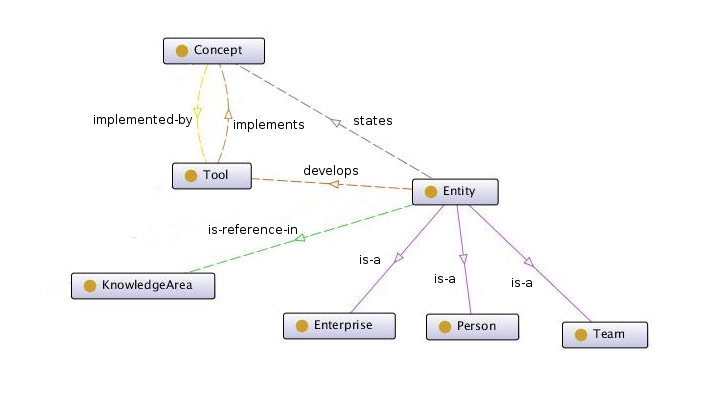
\includegraphics[scale=0.5]{images/onto_entity_relations.jpg}
        \caption{La clase \textit{Entity}}
        \label{entityRelations}
    \end{center}
\end{figure}

La clase \textit{Entity}, envuelve a las clases \textit{Person}, \textit{Team} y \textit{Enterprise}. Según lo expresado en la Figura~\ref{entityRelations} una instancia de \textit{Entity} puede enunciar (\textit{states}) un concepto, desarrollar (\textit{develops}) una herramienta o ser referencia (\textit{is-reference-in}) en un área de conocimiento. Por herencia, cualquier sub-clase de \textit{Entity} será capaz de hacer lo mismo. Adicionalmente, se asocian herramientas (\textit{Tool}) a conceptos (\textit{Concept}) con la finalidad de poder expresar que una herramienta, implementa en la práctica un concepto teórico, por ejemplo: \textit{Python} es un \textit{Lenguaje de Programación} que abarca los paradigmas \textit{Estructurado}, \textit{Orientado a objetos} y \textit{Funcional}, todos estos, serían conceptos y \textit{Python} la herramienta que los implementa. Esto se modela para brindar una mayor expresividad al vocabulario creado a manera de poder satisfacer consultas del tipo ``Herramientas de \textit{Google} para \textit{Cloud Computing}'', por dar un ejemplo.

La clase \textit{Resource}, modela los recursos que hacen referencia a alguna otra clase del modelo de conocimiento generado. Es por ello que cualquier entidad de la \textit{Ontología} puede tener un recurso asociado y, un recurso, puede estar asociado a un concepto si es muy específico, a un área de conocimiento si es más general o, incluso, a la disciplina si es lo suficientemente global como para abarcar toda su extensión, ver Figura~\ref{resourceClass}.

\newpage
\begin{figure}[!h]
    \begin{center}
        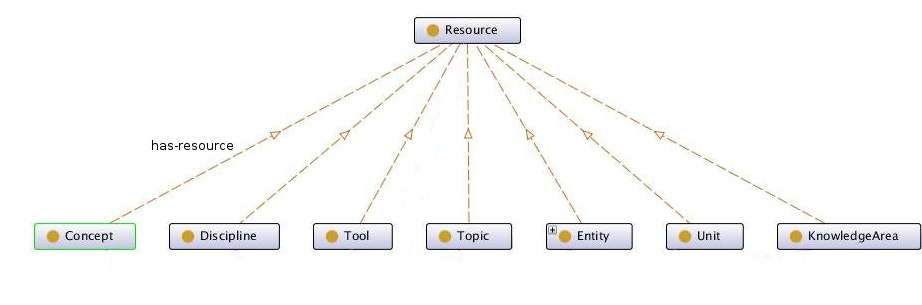
\includegraphics[scale=0.5]{images/onto_resource_class.jpg}
        \caption{La clase \textit{Resource}}
        \label{resourceClass}
    \end{center}
\end{figure}

\subsubsection{Implementación}
Para la implementación de la \textit{Ontología}, se utilizó el editor gráfico \textit{Protègè}, este editor permite la construcción de la \textit{Ontología} de manera gráfica, para ello, se reprodujo el modelo mostrado en la sección anterior y se aprovechó la capacidad de la herramienta para la generación de código. Se realizaron las configuraciones necesarias para que el código se genere con la sintaxis RDF/XML.

Se crearon instancias desde la clase \textit{Discipline} hasta la clase \textit{Topic}, según las áreas de conocimiento, unidades y tópicos especificados en los documentos de recomendación de la \textit{IEEE-CS} y la \textit{ACM}, tomando en cuenta sólo los contenidos del núcleo de la carrera.

Se definieron las relaciones entre las clases y sus reglas de inferencia a través de propiedades \textit{OWL}. Normalmente, cuando se desarrollan bases de conocimiento, se definen los hechos y las reglas de inferencia de manera independiente, en la \textit{Web Semántica}, las reglas de inferencia, como se observó en la etapa de diseño, se encuentran \textbf{dentro} del mismo modelo, mediante la especificación de propiedades lógicas a las relaciones que conectan las clases. Vale destacar que, aún cuando normalmente basta con las propiedades existentes en el vocabulario \textit{OWL}, existen reglas de inferencia que escapan al alcance de estas propiedades, para estos casos es posible escribir un conjunto de reglas utilizando un lenguaje especial para ello llamado \textit{Semantic Web Rule Language} (SWRL). Este lenguaje fue creado para solventar una carencia de \textit{OWL}, al no soportar propiedades compuestas (Hebeler et al, 2009).

\subsubsection{Validación}
Para llevar a cabo la validación de la \textit{Ontología}, se utilizaron dos métodos para determinar dos factores distintos acerca del modelo: 

\begin{itemize}
    \item \textbf{OntoClean:} una metodología propuesta por Guarino y Welty (s/f) para la generación de \textit{Ontologías Limpias}, es decir, con una estructura coherente y consistente. En este caso, se utilizó para validar la estructura, es decir, si las decisiones tomadas respecto a las entidades que fueron modeladas como clases, propiedades e individuales (instancias de clase) fueron acertadas.
    \item \textbf{Domain Questions:} o \textit{Preguntas de Dominio}, es un método propuesto en el texto \textit{Semantic Web for the Working Ontologist}, en el que se realiza una serie de preguntas que el modelo en cuestión debe ser capaz de responder, ya sea por sí solo o a través de inferencia sobre las relaciones y propiedades de cada entidad. Con este método, se busca validar la completitud de la \textit{Ontología}, es decir, si con lo que está expresado en ella, es suficiente para cumplir con el propósito del dominio para el cual fue hecha.
\end{itemize}

\section{[Iteración 5]: Desarrollo de la herramienta para administrar la ontología}
Durante esta etapa, se desarrolló una herramienta para gestionar la ontología desarrollada en la iteración anterior. Esta herramienta no pretende ser un editor de ontologías, pues no editará ni agregará clases ni relaciones.

A través de esta herramienta podrá agregarse nuevos recursos y nuevas instancias a las clases ya creadas y, además, actualizar la ontología razonada dentro del motor de persistencia, cumpliendo de esta manera con el desarrollo de un proceso semiautomático para el crecimiento de la ontología.

Cuando se habla de procedimientos semiautomáticos, se infiere que una parte del proceso se realiza de manera manual, mientras que la otra es llevada a cabo por una agente de software. En este caso, la parte manual del proceso es detectar las nuevas instancias que serán creadas, es decir, los nuevos elementos que serán añadidos al vocabulario, una vez definidos, pueden ser agregados al modelo y persistidos de manera automática a través de la herramienta desarrollada en esta iteración indicando únicamente el nombre y las relaciones de la nueva instancia a través de las opciones propuestas por la herramienta. De la misma manera, a través del motor de inferencia, puede hacerse crecer la ontología escrita en el documento \textit{OWL}, mediante el descubrimiento de nuevas relaciones inferidas a partir de las escritas en el modelo.

Finalmente, vale destacar que dado carácter experimental y prototípico del presente trabajo, se prestará especial atención al procesamiento de los datos en términos de sus relaciones, dejando en segundo plano aspectos como usabilidad, seguridad y diseño a nivel gráfico, tópicos importantes para cualquier sistema completo y que, sin lugar a dudas, deben estar presentes en la solución final pero que fueron relegados a un segundo plano para la presentación de este prototipo y se espera que dichas características sean agregadas en trabajos futuros.

\subsection{Desarrollo de las tareas}
Esta herramienta fue desarrollada utilizando \textit{Java} como lenguaje de programación y \textit{Java Server Pages} (JSP) como herramienta para la generación de vistas web. Como motor de persistencia se utilizó \textit{Virtuoso Open Source Edition}, se utilizó \textit{Pellet} para razonar sobre la ontología y las clases provistas por \textit{Jena} para llevar a cabo la integración de todas estas tecnologías y manipular la ontología subyacente escrita en OWL.

\subsubsection{Análisis}
La herramienta desarrollada es capaz de:

\begin{enumerate}
    \item Agregar, eliminar, consultar y editar recursos.
    \item Agregar, eliminar, consultar y editar anotaciones.
    \item Aplicar razonamiento al modelo a través de un motor de inferencia.
    \item Actualizar el modelo de conocimiento que persiste en \textit{Virtuoso}
\end{enumerate}

Respecto a las clases y las relaciones definidas en la ontología base, una vez que el conocimiento ha sido modelado, es realmente difícil que aparezca información nueva para ser incorporada a nivel de clases. Es por ello que no se incorporó esta funcionalidad en la herramienta, de ocurrir esto, resulta más conveniente agregar las nuevas clases a través de un editor de ontologías especializado (como \texrit{Protègè}). Lo que sí es posible es la aparición de nuevos conceptos o áreas de conocimiento dentro del campo que se realiza el modelo de conocimiento, estos pueden ser agregados como instancias de las clases ya creadas.

\subsubsection{Diseño}
La arquitectura de la herramienta es una fusión de una Arquitectura centrada en datos y una Arquitectura por capas.  

Una Arquitectura centrada en datos (Data Centered Architecture) es aquella en la que los datos son el corazón del sistema y las aplicaciones acceden a ellos para consultarlos y manipularlos o modificarlos según sea el caso, por otra parte, una Arquitectura por capas (Layered Architecture), es aquella en la que se divide la aplicación en distintas capas funcionales, donde las capas más internas realizan operaciones con el sistema operativo, mientras las más externas interactúan con el usuario final (Pressman, 2010)

En este caso, la herramienta modifica, consulta y manipula datos almacenados en documentos OWL y en el motor de persistencia Virtuoso, además, está dividida en tres (3) capas cada vez más cercanas a los datos, en las que la más interna realiza la extracción y escritura de los mismos a través de las clases provistas por \textit{Jena}. La capa intermedia, convierte los datos complejos de que recibe de la capa inferior a algo más simple y fácil de manipular, así como también, realiza el proceso inverso. Finalmente, la capa más externa, está compuesta por archivos JSP y clases Servlet que gestionan las vistas, muestran información e interactúan con el usuario. Se destinó, además, un paquete aislado para las pruebas unitarias.

En la Figura~\ref{adminClassDiagram}, puede observarse la arquitectura diseñada para la herramienta, el funcionamiento se explicará posteriormente en la etapa de implementación.

\newpage

\begin{figure}[!h]
    \begin{center}
        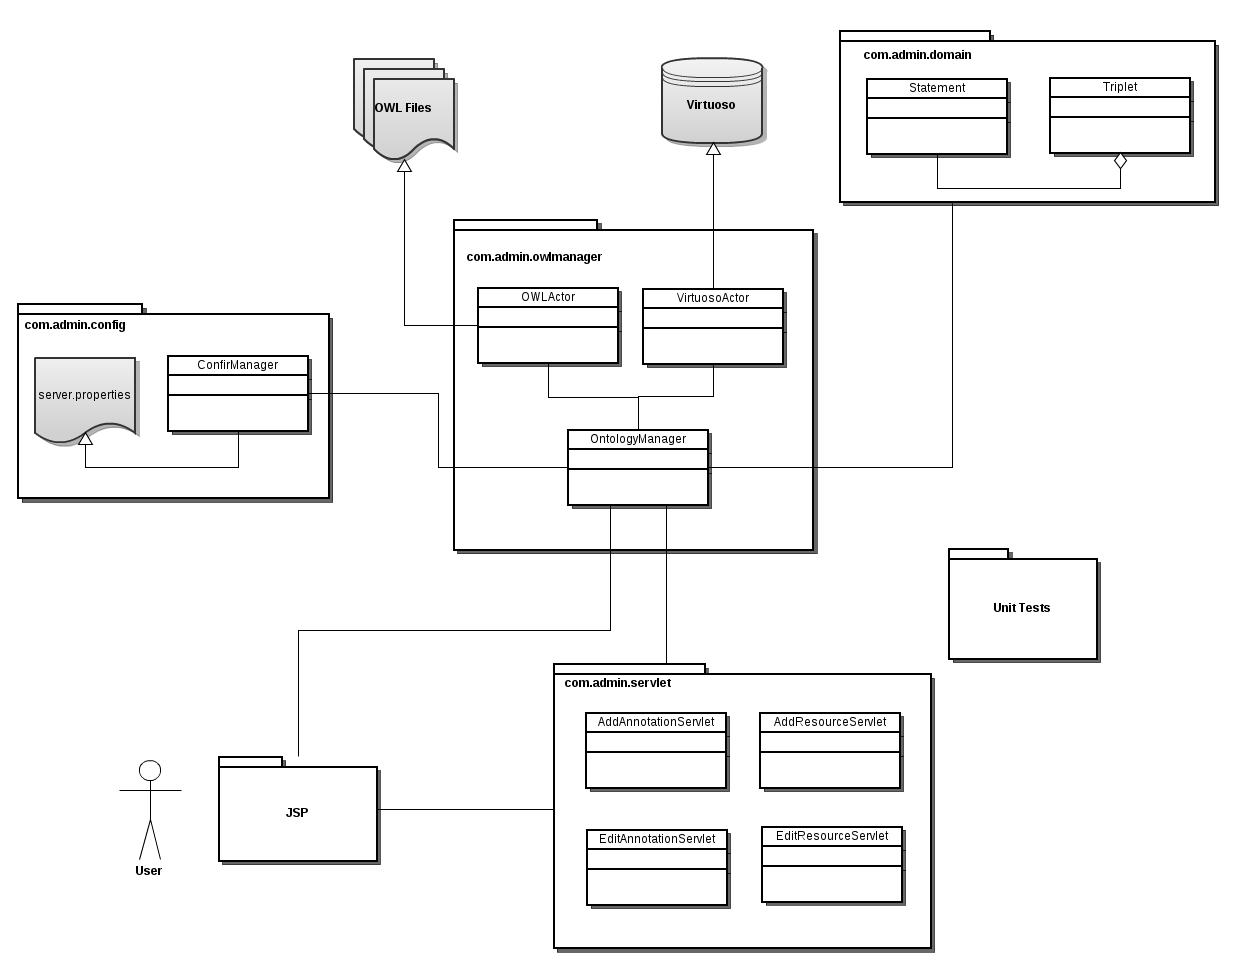
\includegraphics[scale=0.4]{images/admin_app_class_diagram.jpg}
        \caption{Diagrama de clases}
        \label{adminClassDiagram}
    \end{center}
\end{figure}

\subsubsection{Implementación y validación}
Toda la codificación de la herramienta se llevó a cabo utilizando la perspectiva \textit{Java EE} (Java Enterprise Edition) de \textit{Eclipse IDE}, esta perspectiva es la que contiene los módulos necesarios para el desarrollo de aplicaciones web.

Al inicio, se configuró el classpath del proyecto con las librerías del JDK y se incluyeron los paquetes precompilados (paquetes \textit{jar}) necesarios para el funcionamiento correcto de \textit{Jena Framework} y el motor de inferencia \textit{Pellet}, así como también el driver JDBC para \textit{Virtuoso}. 

Las clases que conforman la arquitectura diseñada en la etapa anterior, tienen, en líneas generales las siguientes funciones:

\begin{itemize}
    \item Las clases \textit{OWLActor} y \textit{VirtuosoActor} interactúan con los medios de persistencia en OWL y Virtuoso respectivamente, extrayendo, escribiendo o actualizando datos, según sea el caso, retorna los datos con los tipos tal como son extraídos de su medio de persistencia.
    \item La clase \textit{OntologyManager} es la encargada de realizar la transformación de los datos complejos que proveen las clases \textit{OWLActor} y \textit{VirtuosoActor} como las distintas abstracciones de recursos como las clases \textit{Individual}, \textit{Resource}, \textit{RDFNode} y \textit{Property} de \textit{Jena} a los \textit{JavaBeans} \textit{MyStatement} y \textit{Triplet}, definidos en el paquete \textit{com.admin.domain}, así como de realizar transformaciones de colecciones abstractas como el \textit{StmtIterator} a colecciones más manejables y conocidas como el \textit{TreeSet} y el \textit{ArrayList} de \textit{Java}, estos \textit{JavaBeans} y estas colecciones, son más manejables para la capa de presentación. La clase \textit{OntologyManager} también realiza el proceso inverso de conversión y la extracción de las propiedades de configuración mediante llamadas a la clase \textit{ConfigManager}, destinada a interactuar con el archivo de configuración. En pocas palabras, \textit{OntologyManager} orquesta los métodos escritos en las clases subyacentes para satisfacer las peticiones enviadas desde las vistas.
    \item A nivel de vistas, para mostrar datos, la información va directamente desde la clase \textit{OntologyManager}, pero en el caso contrario, es decir, cuando una vista necesita comunicarse con \textit{OntologyManager}, no lo hace directamente, la solicitud es procesada por un \textit{Servlet} que despacha la operación a los métodos correctos de \textit{OntologyManager} según el evento que se haya invocado en la vista JSP activa.

\end{itemize}

El desarrollo se dividió por características en forma de historias de usuario y fueron desarrolladas en el siguiente orden:

\begin{enumerate}
    \item Yo como \textbf{usuario}, deseo poder crear recursos \textbf{para} enriquecer la ontología y extender los resultados de búsqueda.
    \item Yo como \textbf{usuario}, deseo poder modificar recursos previamente creados \textbf{para} corregir errores en el etiquetado de manera fácil y mejorar los resultados de búsqueda.
    \item Yo como \textbf{usuario}, deseo poder eliminar recursos \textbf{para} mantener la ontología limpia de recursos obsoletos o inexistentes.
    \item Yo como \textbf{usuario}, deseo poder crear anotaciones \textbf{para} extender el vocabulario de la ontología e incluir nuevos conceptos.
    \item Yo como \textbf{usuario}, deseo poder modificar anotaciones \textbf{para} corregir errores en el vocabulario y evitar resultados de búsqueda inconsistentes.
    \item Yo como \textbf{usuario}, deseo poder eliminar anotaciones \textbf{para} mantener la ontología limpia de conceptos no vigentes o descritos de manera errada.
\end{enumerate}

Cada característica fue desarrollada ``de abajo hacia arriba'', es decir, codificó en primera instancia los métodos de extracción y/o escritura de datos en las clases \textit{OWLActor} o \textit{VirtuosoActor} según fuera el caso y se validaba su correcto funcionamiento mediante \textit{Pruebas Unitarias} a través de \textit{JUnit Framework}, luego se codificaba la lógica de traducción de los datos provistos por la capa de persistencia a los definidos en en paquete \textit{com.admin.domain} y el proceso inverso, así como las transformaciones necesarias para proveer datos que fueran lo más fáciles de manejar posible a la capa de presentación. Luego de eso, se construía la vista básica de los datos, la cual se enriquecía poco a poco utilizando \textit{CSS} para mejorar el estilo de la presentación de los datos y \textit{JavaScript} para realizar peticiones de datos asíncronas al servidor en los casos que hiciera falta. Finalmente, se codificaba la lógica de envío de datos en los \textit{Servlets} correspondientes.

Únicamente se desarrollaron pruebas unitarias para los métodos de persistencia y en algunos de la capa de transformación, pues no en todos la lógica era lo suficientemente compleja como para requerir validar su funcionamiento a través de este método.

\section{[Iteración 6]: Desarrollo del buscador}
En esta iteración se describe el desarrollo del buscador como tal, su diseño y su implementación utilizando \textit{Python}. Debido al carácter experimental y prototípico de este trabajo, aspectos como usabilidad y diseño gráfico fueron dejados en segundo plano para concentrar la atención en el procesamiento de la información y en el desarrollo de algoritmos que ejecuten las tareas de manera eficiente.

\subsection{Desarrollo de las tareas}
El buscador fue desarrollado utilizando \textit{Python} como lenguaje de programación, el módulo \textit{CherryPy} para la generación de vistas web, un protocolo de comunicación basado en \textit{JSON} para la comunicación con el \textit{endpoint} de \textit{SPARQL} que provee \textit{Virtuoso}, encapsulado dentro del módulo \textit{sparql-wrapper}, y el módulo \textit{Python Lex-Yacc} (PLY) para diseñar un lenguaje de consultas basado en anotaciones y conectores lógicos amigable para el usuario, intuitivo y que, a partir de esa gramática, se pudiera generar la o las sentencias \textit{SPARQL} necesarias para satisfacer la consulta del usuario, finalmente, se utilizó el \textit{framework} para desarrollo web \textit{CherryPy}, junto con el lenguaje de plantillas de \textit{Mako Templates} para generar las vistas del buscador, nuevamente, debido al carácter prototípico de este trabajo, el diseño y aspecto visual, pasan a un segundo plano, prevaleciendo el procesamiento de los datos como prioridad en este desarrollo.

\subsubsection{Análisis}
El buscador, es un sistema completo que debe recibir consultas, procesarlas, solicitar la información necesaria al medio de persistencia a través de sentencias \textit{SPARQL} y mostrar los resultados al usuario. Este requerimiento general, puede ser separado en las siguientes historias de usuario:

\begin{enumerate}
    \item Yo como \textbf{usuario} requiero un sistema que procese mis consultas \textit{para} conseguir recursos en el área de Ciencias de la Computación de manera sencilla.
    \item Yo como \textbf{desarrollador} requiero de un componente que separe la consulta del usuario en partes más manejables \textbf{para} poder procesarla fácilmente.
    \item Yo como \textbf{desarrollador} requiero de un componente que traduzca la consulta del usuario a lenguaje \textit{SPARQL} \textbf{para} poder realizar solicitudes al medio de persistencia.
\end{enumerate}

El buscador debe ser capaz de satisfacer distintos tipos de consultas, pueden clasificarse en tres (3) grupos:

\begin{enumerate}
    \item Consultas en las que se requiere que un recurso posea un conjunto de anotaciones específicas.
    \item Consultas en las que se requiere que un recurso posea un conjunto de anotaciones específicas u otro.
    \item Consultas de tópicos relacionados a una anotación específica.
\end{enumerate}

Estas consultas se hacen a través del lenguaje \textit{SPARQL}, este es un lenguaje formal en el que no resulta conveniente obligar al usuario a escribir pues, si bien su curva de aprendizaje no es muy empinada, el objetivo es realizar búsquedas utilizando tecnologías de \textit{Web Semántica} de manera sencilla, si quisiéramos que el usuario introdujera consultas utilizando \textit{SPARQL} en nuestro buscador, con el \textit{endpoint} que provee \textit{Virtuoso} sería más que suficiente.

\subsubsection{Diseño}
Para empezar el desarrollo del buscador, debe resolverse primero el problema de cómo se realizarán las consultas.

Dado que el \textit{Procesamiento de Lenguaje Natural} es un tema que excede el alcance de este trabajo, se decidió diseñar un lenguaje formal y, al mismo tiempo, ``amigable al usuario'' para la escritura de las consultas. Este lenguaje está basado en anotaciones conectadas a través de conectores lógicos \textit{OR}, \textit{AND} y \textit{NOT}, además de un operador para calcular los tópicos relacionados a una anotación dada, el operador \textit{?rel:}.

Para procesar las consultas en el lenguaje lógico, se asume que todas las consultas lingüísticas pueden escribirse, de manera formal, en \textit{Forma Normal Disyuntiva} (DNF) o en \textit{Forma Normal Conjuntiva} (CNF) (Luque et al, s/f), diseñando, para este caso, una gramática que soporte la escritura de consultas en un lenguaje lógico formal en DFN.

\begin{figure}[!h]
    \begin{center}
        \begin{verbatim} 
            Query     : OrQuery | AndQuery
            OrQuery   : AndQuery \|\| OrQuery | AndQuery
            AndQuery  : AndQuery && UnitQuery | UnitQuery
            UnitQuery : Annotation | \?rel: Annotation | \- Annotation
        \end{verbatim}
        \caption{Gramática del lenguaje en notación BNF}
        \label{BNFGrammar}
    \end{center}
\end{figure}

En la Figura~\ref{BNFGrammar}, se aprecia la gramática formal del lenguaje de consultas diseñado, se define un \textit{Query unitario} (UnitQuery) como aquel conformado por sólo una anotación o por una consulta de tópicos relacionados. La gramática expuesta en la Figura~\ref{BNFGrammar} se traduce en lo siguiente:

\begin{itemize}
    \item Un \textit{Query}, está conformado por una solicitud de tipo \textit{OR} (OrQuery) o una solicitud de tipo \textit{AND} (AndQuery).
    \item Un \textit{OrQuery} está conformado por un \textit{AndQuery} en disyunción con un \textit{OrQuery} o un \textit{AndQuery}.
    \item Un \textit{AndQuery} está conformado por un \textit{AndQuery} en conjunción con un \textit{UnitQuery} o un \textit{UnitQuery}.
    \item Un \textit{UnitQuery} está conformado por una anotación o por un query de tipo \textit{?rel:} o por un query de tipo \textit{NOT}.
\end{itemize}

Esta gramática, primero separa todas las disyunciones de la consulta y las agrupa en consultas individuales conjuntivas, separadas por disyunciones, es decir, el lenguaje diseñado procesa consultas en DNF.

El componente diseñado corresponde al lo escrito en la historia de usuario número dos, pues toma la consulta y la separa en partes que pueden ser procesadas y traducidas posteriormente de manera más sencilla. La arquitectura completa del buscador, se presenta en la Figura~\ref{searcher_architecture}

\begin{figure}[!h]
    \begin{center}
        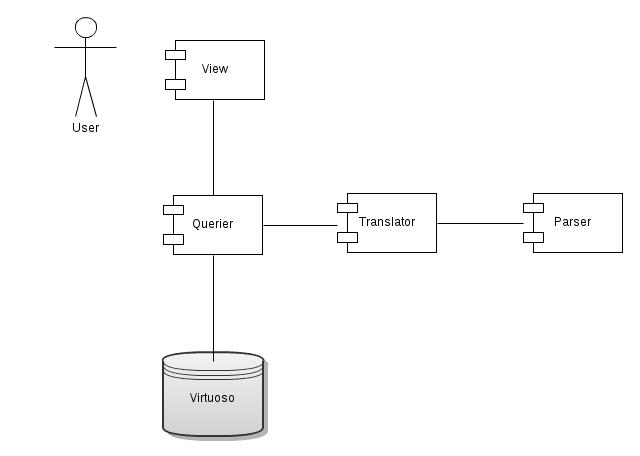
\includegraphics[scale=0.4]{images/searcher_components.jpg}
        \caption{Diagrama de componentes}
        \label{searcher_architecture}
    \end{center}
\end{figure}

\subsubsection{Implementación y validación}
Toda la codificación del prototipo del sistema de búsqueda se llevó a cabo utilizando el editor \textit{VIM} (Vi Improved) con la extensión \textit{NERDTree} para navegar a través de los directorios del proyecto y abrir archivos de código fuente en pestañas distintas dentro de la misma instancia del editor en la misma línea de comandos.

La primera etapa del desarrollo, se enfocó en el \textit{Parser} para el lenguaje diseñado, para ello se utilizó el módulo \textit{Python Lex-Yacc} (PLY), que permite escribir compiladores e intérpretes para gramáticas libres de contexto, que es el basamento de los lenguajes formales. PLY, contiene dos clases: \textit{lex} y \textit{yacc} que son, respectivamente, un analizador léxico y un parser.

El analizador léxico, conocido también como \textit{lexer}, separa la entrada en partes conocidas como \textit{tokens}, cada vez que el \textit{lexer} retorna un \textit{token}, lo asocia con un componente léxico del lenguaje o \textit{lexema} (Aho et al, 2007), es decir, este análisis léxico de cada expresión, comprende la separación y clasificación de cada parte de dicha expresión en componentes léxicos conocidos por el intérprete.

En este caso, el \textit{lexer} debe reconocer cinco (5) \textit{lexemas} básicos: \textit{AND}, \textit{OR}, \textit{NOT} y \textit{REL}, que son los operadores sobre el quinto \textit{lexema} que compone el lenguaje: \textit{ANNOTATION}. Estos componentes léxicos se describen, a nivel de código fuente, a través de expresiones regulares. Como el público objetivo de este sistema son personas del área de Ciencias de la Computación, los símbolos para los \textit{lexemas} \textit{AND} y \textit{OR} son las secuencias de caracteres \textit(doble ampersand) y \textit{doble barra vertical} respectivamente pues son los símbolos para los operadores lógicos ``y'' y ``o''en muchos lenguajes de programación ampliamente utilizados y difundidos como \textit{C}, \textit{Java} y \textit{PHP}, por lo que debería resultar intuitivo para estas personas la utilización de esa simbología. Por otra parte, el operador \textit{?rel:} debería leerse como ``pregunta por lo relacionado a:'', es por ello que se seleccionó esa secuencia de caracteres, finalmente, el operador \textit{NOT}, está representado por el operador aritmético de sustracción.

Una consulta utilizando este lenguaje debería lucir como lo escrito en la Figura~\ref{SimpleQueryExample}

\begin{figure}[!h]
    \begin{center}
        \begin{verbatim}
        web services && java || web services && python && -SOAP
        \end{verbatim}
        \caption{Ejemplo de query utilizando el lenguaje especificado}
        \label{SimpleQueryExample}
    \end{center}
\end{figure}

Respecto a consultas ilegales, un query de tipo \textit{NOT} generará un error si no está dentro de un query de tipo \textit{AND}, esto es porque internamente al interpretar la consulta, el query de negación es interpretado como un modificador \textit{FILTER} al ser traducido a \textit{SPARQL}. De la misma manera, una conjunción de expresiones \textit{?rel:} no está permitida pues el intérprete, en tiempo de traducción, calcula los elementos relacionados a la anotación que acompaña al operador y genera una expresión de tipo \textit{OR} con dichos elementos.

El parser, por otra parte, realiza un análisis sintáctico, aplicando las reglas gramaticales definidas anteriormente. Este proceso de interpretación del lenguaje lleva a cabo estas dos etapas, el proceso de traducción, toma el árbol sintáctico que construye el parser y lo recorre de manera recursiva, traduciendo esas expresiones en consultas \textit{SPARQL} que son enviadas al medio de persistencia a través del módulo de \textit{Python} \textit{sparql-wrapper}.

Finalmente, toda la capa de presentación, fue desarrollada utilizando el módulo \textit{CherryPy}, que constituye un \textit{framework} sencillo para aplicaciones web, no incluye ninguna herramienta \textit{ORM} (Object-Relational Maping), lo que resulta conveniente ya que nuestra fuente de datos no es una Base de Datos Relacional, ni una herramienta de plantillas, por ello, se seleccionó \textit{Mako Templates} para el diseño de las vistas. Tomando el cuenta el carácter prototípico y experimental de este trabajo, el diseño gráfico y los aspectos de usabilidad fueron relegados a un segundo plano. Toda la validación del software, se llevó a cabo mediante la escritura de \textit{Pruebas Unitarias} a través del framework \textit{unittest}, que sigue una filosofía muy similar al framework \textit{JUnit}, utilizado para validar el funcionamiento correcto de los componentes de la herramienta de administración de la ontología desarrollada en la iteración anterior.


\newpage
